
\begin{center}\texttt{5 - Monitoring and Control}\end{center}
\hrulefill \\

\noindent How is the project going? Is our plan being respected? If not, react! How to react? 

\noindent Monitoring: collecting data on the prj execution, depending on what you want to check;

\noindent Control: comparing the collected data to the plan, establish if you're in line with the plan.

\noindent Projects misalign to the plan in 4 main ways:
\begin{itemize}
    \item delays in meeting target deadlines: same feature but at a different (later) time;
    \item shortfall in quality: your product is not of the quality you had planned, usually due to a lack of QA activities you might've skipped to save time;
    \item inadequate functionality: we don't have the exact amount and type of functionalities we wanted (bad requirement gathering activity, probably!!). In a way, this is the same problem as having delays;
    \item cost over target - in a way, a consequence of all three;
\end{itemize}

\noindent Communication Infrastructure: if you need to collect data, you need to know who to ask. This usually goes together with the hierarchy of responsibilities within the company, i.e.: 

\begin{figure} [H]
    \centering
    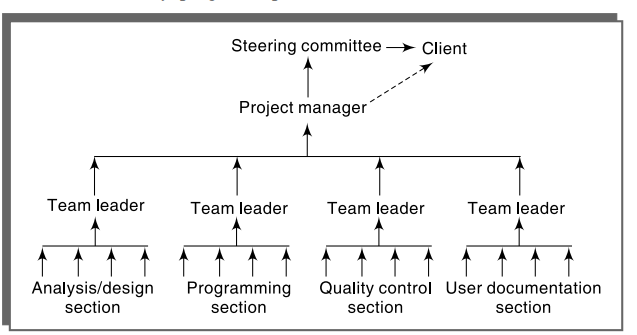
\includegraphics[width=0.75\linewidth]{Figures//06/randc.png}
    \caption{Who reports to who? What do you ask who?}
\end{figure}

\noindent Reporting to your immediate supervisor should be done in a planned way, could be written or oral, could be formal or informal, could be regular or ad-hoc (kinda like planned or upon need). Written reports are usually formal. Oral, formal, regular makes for a regular meeting, a checkpoint previously added in the plan. Job sheets are used to keep track of what people are working on throughout a week, progress reports are written by the team to describe what they have been doing, these are more about the work than about the people.

\begin{figure} [H]
    \centering
    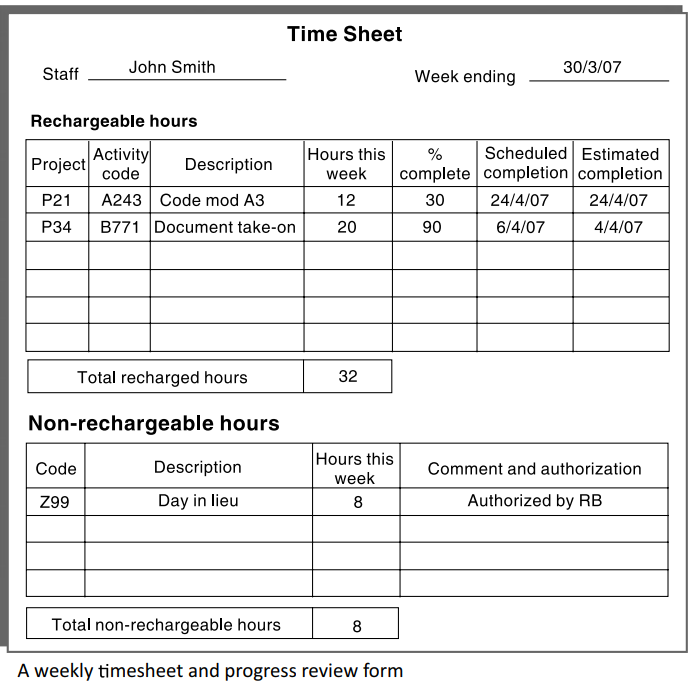
\includegraphics[width=0.5\linewidth]{Figures//06/weeklytimesheet.png}
\end{figure}

\noindent From such a report, you can get information such as: the pace of this worker is somewhat slow, monitor the situation in case things don't speed up or some other issue is underlying.

\noindent Red/Amber/Green (or traffic light) reporting: ask the worker the sitrep about the activities and the likelihood of meeting target dates, estimate the risk of being late basically. ``Green'' is all good, ``Amber'' just keep monitoring, ``Red'' we will be late for sure, react to this information asap! Assign more people or something like that. Also depends on the criticality of the activity in question.

\noindent You can use Gantt charts in a dynamic way to compare the bars of the plan with dynamic bars of what you have done so far!

\begin{figure} [H]
    \centering
    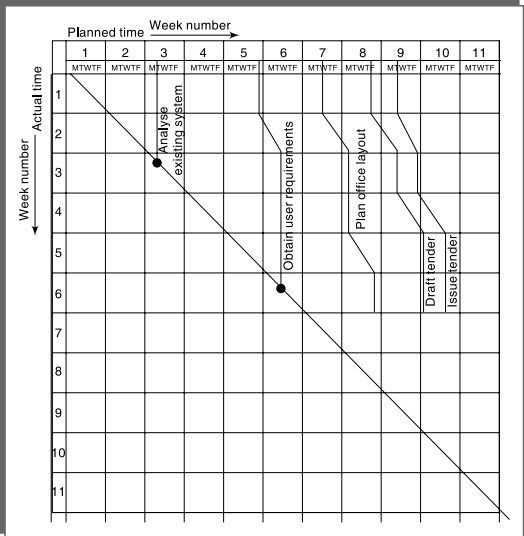
\includegraphics[width=0.5\linewidth]{Figures//06/timeline.png}
    \caption{Monitoring time of project with respect to the plan}
\end{figure}

\begin{figure} [H]
    \centering
    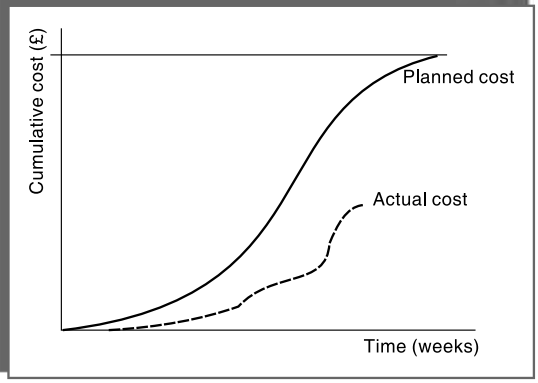
\includegraphics[width=0.75\linewidth]{Figures//06/costmonitoring.png}
    \caption{Plotting the comparison of estimated vs actual cost over time. Cost can be compared to the actual value. The cumulative expenditure chart (not this one) can also show revised es mates of cost and completion date.}
\end{figure}

\noindent Earned Value at some day D: different strategies to estimate earned value; happens at different percentages at various stages, 0/100 is about start/end difference, nothing in the middle; 50/50 you acquire 50 when you start and 50 when you end the activity; 75/25; or it's milestone based, you acquire value upon reaching a checkpoint; percentage-complete is less reliable.

\noindent Indexes:

\begin{itemize}
    \item Schedule Variance: EV - PV, earned value - planned value;
    \item time variance;
    \item cost variance CV = EV -AC; earned value minus actual cost;
    \item performance ratios: Cost performance index = $\dfrac{EV}{AC}$; schedule performance index = $\dfrac{EV}{PV}$
\end{itemize}

\begin{figure} [H]
    \centering
    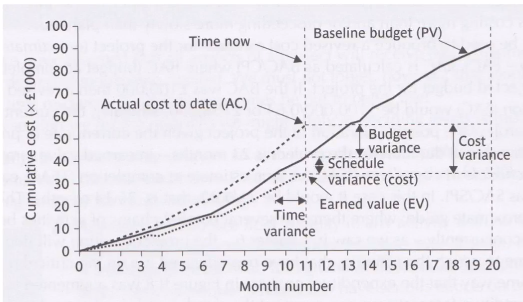
\includegraphics[width=0.75\linewidth]{Figures//06/indexes.png}
\end{figure}


\noindent CPI can be used to make a projection forward, an Estimate At Completion EAC = $\dfrac{BAC}{CPI}$ with BAC being Budget at Completion. If things are especially bad and you realize you cannot afford it, welp you might want to drop it! If you're above 20\% that's catastrophe :D

\noindent Monitor more the critical activities, activities with no free float, those with little float, those with critical resources.

\noindent Once you notice a misalignment, you can take action: intervene on the critical path, i.e. add resources, increase work hours or reorganize the team, reduce scope (less functionalities) or reduce quality. Or you reconsider the plan, change priority of requirements.

